\documentclass[a4paper, 12pt]{report}
\usepackage{cmap}
\usepackage[T2A]{fontenc}
\usepackage[utf8]{inputenc}
\usepackage[english,russian]{babel}
\usepackage{listings}
\usepackage{amsmath}
\usepackage{float}
\usepackage{csquotes}
\usepackage{graphicx}
\graphicspath{ {./images/} }
\usepackage{xcolor}
\definecolor{buzzlightyear}{HTML}{8757A5}
\definecolor{grass}{HTML}{738D06}
\definecolor{literal}{HTML}{F18A2B}
\definecolor{commentcolor}{HTML}{8E908B}

\lstdefinestyle{habrstyle}{
	backgroundcolor=\color{white},
	commentstyle=\color{commentcolor},
	keywordstyle=\bfseries\color{buzzlightyear},
	numberstyle=\tiny\color{commentcolor},
	stringstyle=\color{grass},
	basicstyle=\ttfamily\footnotesize,
	breakatwhitespace=false,         
    	breaklines=true,                 
   	captionpos=b,                    
    	keepspaces=true,                 
    	numbers=left,                    
    	numbersep=7pt,                  
    	showspaces=false,                
    	showstringspaces=false,
   	showtabs=false,                  
    	tabsize=3
}

\lstset{style=habrstyle}

\author{3530901/80201, Шелаев Н. Р.}
\title{Лабораторная работа № 9. Дифференцирование и интегрирование.}
\date{\today}

\begin{document}
	\maketitle
	\tableofcontents
	\listoffigures
	\lstlistoflistings

	\chapter{Конечные разности}
	Проверим, что вычисление разницы между соседними элементами во временной области соответствуют фильтру ВЧ.
	\begin{lstlisting}[language=Python,caption=И снова акции Facebook]
		import pandas as pd
		from thinkdsp import Wave

		df = pd.read_csv('FB_2.csv', header=0, parse_dates=[0])
		ys = df['Close']
		if len(ys) % 2: ys = ys[:-1]
		close = Wave(ys, framerate = 1)
		close.plot()
		close_spectrum = close.make_spectrum()
		close_spectrum.plot()
	\end{lstlisting}
	\begin{figure}[H]
		\centering
		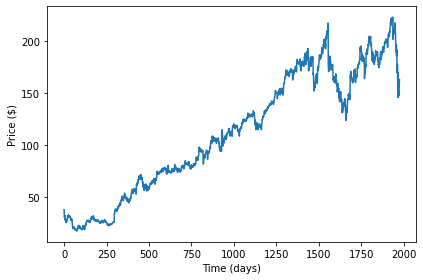
\includegraphics[width=0.75\textwidth]{fac1.png}
		\caption{Сам график}
		\label{fig:fac1}
	\end{figure}
	\begin{figure}[H]
		\centering
		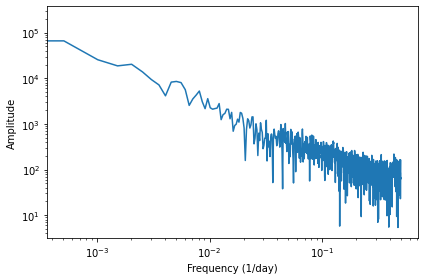
\includegraphics[width=0.75\textwidth]{fac2.png}
		\caption{График в логарифмическом масштабе}
		\label{fig:fac2}
	\end{figure}
	Наклон линии мощности составляет примерно -1.8, что очень близко к \textquote{Красному} шуму (-2).
	\begin{lstlisting}[language=Python,caption=Считаем разницу между последовательными элементами]
		change = Wave(np.diff(close.ys), framerate = 1)
		change.plot()
		change_spectrum = change.make_spectrum()
		change_spectrum.plot()
		decorate(xlabel = 'Frequency (1/day)', ylabel = 'Amplitude')

		change_spectrum.plot()
		decorate(xlabel='Frequency (1/day)', ylabel='Amplitude', xscale='log', yscale='log')
	\end{lstlisting}
	\begin{figure}[H]
		\centering
		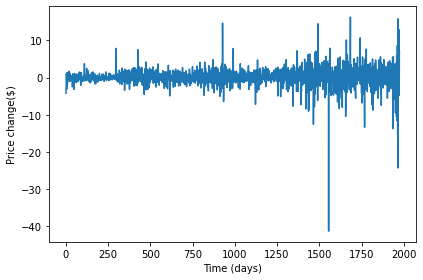
\includegraphics[width=0.75\textwidth]{fac3.png}
		\caption{Разница между ежедневными значениями акций}
		\label{fig:fac3}
	\end{figure}
	\begin{figure}[H]
		\centering
		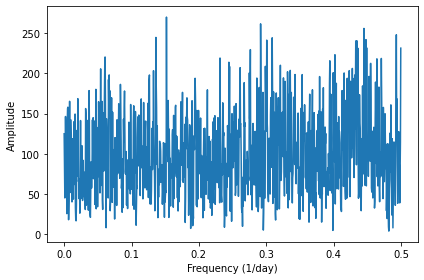
\includegraphics[width=0.75\textwidth]{fac4.png}
		\caption{Спектр ежедневных изменений}
		\label{fig:fac4}
	\end{figure}
	\begin{figure}[H]
		\centering
		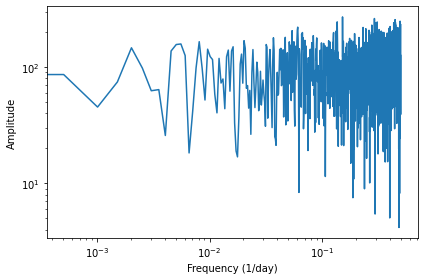
\includegraphics[width=0.75\textwidth]{fac5.png}
		\caption{Спектр в логарифмическом масштабе}
		\label{fig:fac5}
	\end{figure}
	Наклон прямой близок к 0, поэтому можно сделать вывод, что это \textquote{Белый} шум.
	\begin{lstlisting}[language=Python,caption=Умножение на фильтр - свертка с окном]
		from thinkdsp import zero_pad

		def make_filter(window, wave):
			padded = zero_pad(window, len(wave))
			window_wave = Wave(padded, framerate = wave.framerate)
			window_spectrum = window_wave.make_spectrum()
			return window_spectrum

		diff_window = np.array([1.0, -1.0])
		diff_filter = make_filter(diff_window, close)
		diff_filter.plot()
		plt.plot(diff_filter.angles)
	\end{lstlisting}
	\begin{figure}[H]
		\centering
		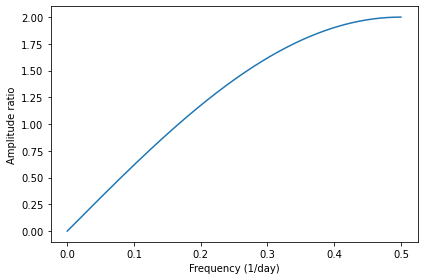
\includegraphics[width=0.75\textwidth]{fac6.png}
		\caption{Фильтр для окна}
		\label{fig:fac6}
	\end{figure}
	\begin{figure}[H]
		\centering
		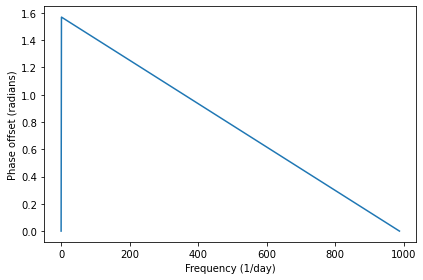
\includegraphics[width=0.75\textwidth]{fac7.png}
		\caption{Углы фильтра}
		\label{fig:fac7}
	\end{figure}
	\begin{lstlisting}[language=Python,caption=Умножаем спектр цен на полученный фильтр]
		change_spectrum2 = close_spectrum * diff_filter
		change_spectrum2.plot()
		change2 = change_spectrum2.make_wave()
		change2.ys = change2.ys[1:]
		change2.ts = change2.ts[1:]
	\end{lstlisting}
	\begin{figure}[H]
		\centering
		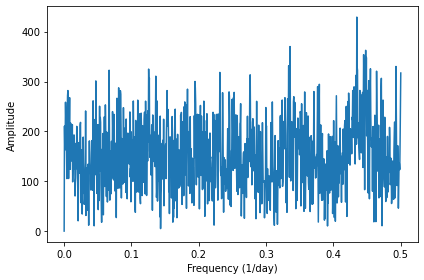
\includegraphics[width=0.75\textwidth]{fac8.png}
		\caption{Изменённый спектр цен}
		\label{fig:fac8}
	\end{figure}
	\begin{figure}[H]
		\centering
		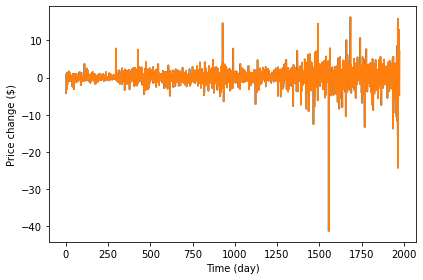
\includegraphics[width=0.75\textwidth]{fac9.png}
		\caption{Сравнение двух ранее полученных методов}
		\label{fig:fac9}
	\end{figure}
	Результаты этих двух методов совпадают.

	\chapter{Дифференцирование}
	Дифференцирование во временной области соответствует простому фильтру в частотной области.
	\begin{lstlisting}[language=Python,caption=]
		PI2 = np.pi * 2
		deriv_filter = close.make_spectrum()
		deriv_filter.hs = PI2 * 1j * deriv_filter.fs
		deriv_filter.plot()
		deriv_spectrum = close.make_spectrum().differentiate()
		deriv_spectrum.plot()
	\end{lstlisting}
	\begin{figure}[H]
		\centering
		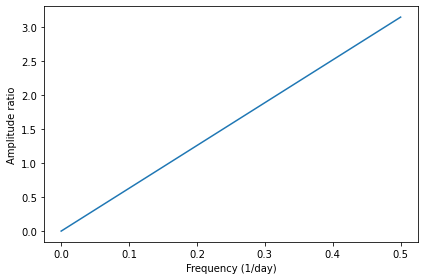
\includegraphics[width=0.75\textwidth]{dif1.png}
		\caption{Фильтр для дифференцирования}
		\label{fig:dif1}
	\end{figure}
	\begin{figure}[H]
		\centering
		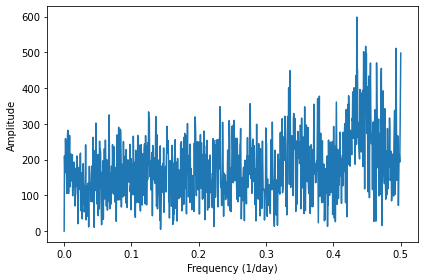
\includegraphics[width=0.75\textwidth]{dif2.png}
		\caption{Результат применения фильтра}
		\label{fig:dif2}
	\end{figure}
	\begin{lstlisting}[language=Python,caption=Сравнение двух методов]
		deriv = deriv_spectrum.make_wave()
		deriv = deriv_spectrum.make_wave()
		change.plot(alpha = 0.5)
		deriv.plot(alpha = 0.5)
	\end{lstlisting}
	\begin{figure}[H]
		\centering
		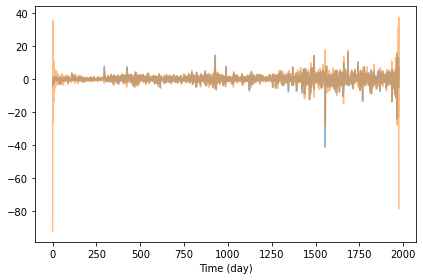
\includegraphics[width=0.75\textwidth]{dif3.png}
		\caption{Результаты этих методов похожи}
		\label{fig:dif3}
	\end{figure}
	Полученные результаты совпадают с \sloppy{\texttt{np.diff}}, но с некоторой погрешностью: окно разности является лишь грубым приближением производной (особенно, на высоких частотах), и спектральная производная основана на предположении, что сигнал является периодическим (а это не так), поэтому в начале и в конце окна поведение отличается.
	\begin{lstlisting}[language=Python,caption=Увеличим масштаб]
		low, high = 0, 50
		plt.plot(change.ys[low:high], label = 'diff')
		plt.plot(deriv.ys[low:high], label = 'deriv')
		deriv_filter.plot()
		diff_filter.plot()
	\end{lstlisting}
	\begin{figure}[H]
		\centering
		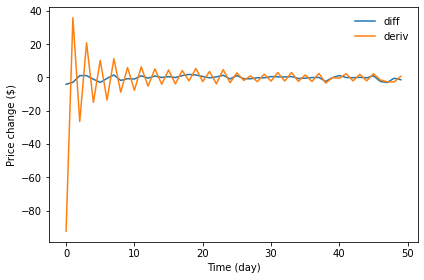
\includegraphics[width=0.75\textwidth]{dif4.png}
		\caption{Теперь лучше видны различия}
		\label{fig:dif4}
	\end{figure}
	\begin{figure}[H]
		\centering
		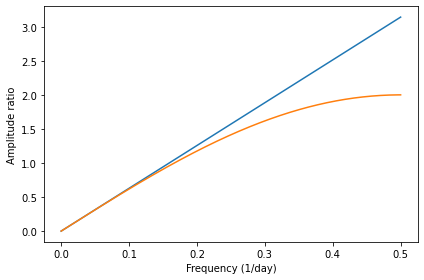
\includegraphics[width=0.75\textwidth]{dif5.png}
		\caption{Разница между фильтром для дифференцирования и разностным фильтром}
		\label{fig:dif5}
	\end{figure}	
	Разностный фильтр не так сильно усиливает высокие частоты.

	\chapter{Интегрирование}
	Поскольку интегрирование обратно дифференцированию, оно также соответствует простому фильтру.
	\begin{lstlisting}[language=Python,caption=Фильтр для интегрирования]
		integ_filter = deriv_filter.copy()
		integ_filter.hs[1:] = 1/(PI2*1j*integ_filter.fs[1:])
		integ_filter.hs[0] = np.inf
		integ_filter.plot()
	\end{lstlisting}
	\begin{figure}[H]
		\centering
		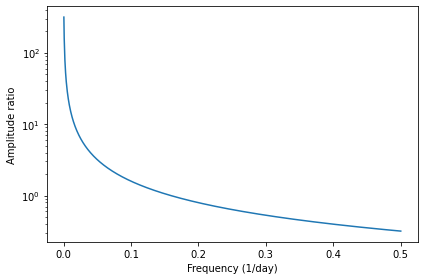
\includegraphics[width=0.75\textwidth]{int1.png}
		\caption{Вид полученного фильтра}
		\label{fig:int1}
	\end{figure}
	\begin{lstlisting}[language=Python,caption=Фильтр для интегрирования]
		integ_spectrum = deriv_spectrum.copy().integrate()
		integ_spectrum.plot()
		close.plot(label = 'closing prices', alpha = 0.7)
		integ_spectrum.hs[0] = 0
		integ_wave = integ_spectrum.make_wave()
		integ_wave.plot(label = 'integrated derivative', alpha = 0.7)
	\end{lstlisting}
		\begin{figure}[H]
		\centering
		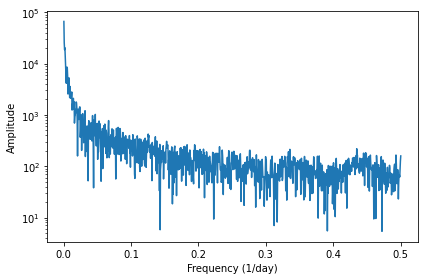
\includegraphics[width=0.75\textwidth]{int2.png}
		\caption{Применим фильтр для спектра производной}
		\label{fig:int2}
	\end{figure}
	\begin{figure}[H]
		\centering
		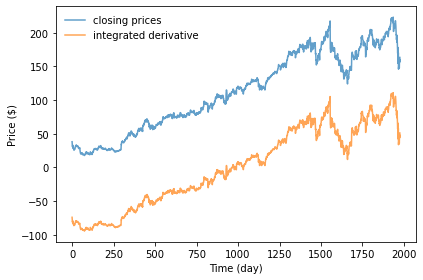
\includegraphics[width=0.75\textwidth]{int3.png}
		\caption{Сравнение исходного сигнала и сигнала после дифференцирования и интегрирования}
		\label{fig:int3}
	\end{figure}
	Результат применения фильтров совпал с исходным графиком, но сдвинут таким образом, что среднее значение равно 0. Производная выбирает первый элемент спектра, который является смещением, а интегрирование не может его восстановить. Поэтому, полученный результат имеет неопределенную константу интегрирования.
	Если сдвинуть полученный результат к исходному, то разница между ними близка к 0.

	\chapter{Нарастающая сумма}
	Оператор \sloppy{\texttt{diff}} аппроксимирует дифференцирование, а нарастающая сумма - интегрирование.
	\begin{lstlisting}[language=Python,caption=Наш любимый пилообразный сигнал]
		from thinkdsp import SawtoothSignal

		in_wave = SawtoothSignal(freq = 50).make_wave(duration=0.1, framerate=44100)
		in_wave.unbias()
		in_wave.plot()
		in_spectrum = in_wave.make_spectrum()
		in_spectrum.plot()
	\end{lstlisting}
	\begin{figure}[H]
		\centering
		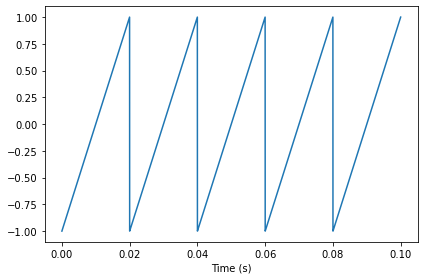
\includegraphics[width=0.75\textwidth]{sum1.png}
		\caption{Вид пилообразного сигнала}
		\label{fig:sum1}
	\end{figure}
	\begin{figure}[H]
		\centering
		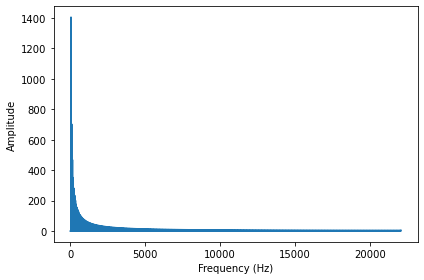
\includegraphics[width=0.75\textwidth]{sum2.png}
		\caption{И его спектр}
		\label{fig:sum2}
	\end{figure}
	\begin{lstlisting}[language=Python,caption=Посчитаем сумму]
		out_wave = in_wave.cumsum()
		out_wave.unbias()
		out_wave.plot()
		out_spectrum = out_wave.make_spectrum()
		out_spectrum.plot()
		ratio_spectrum = out_spectrum.ratio(in_spectrum, thresh=1)
		ratio_spectrum.plot(marker = '.', ms = 4, ls = '')
	\end{lstlisting}
	\begin{figure}[H]
		\centering
		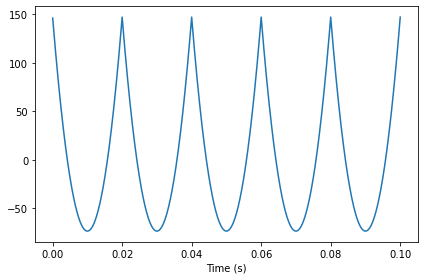
\includegraphics[width=0.75\textwidth]{sum3.png}
		\caption{Получили вот этот сигнал}
		\label{fig:sum3}
	\end{figure}
	\begin{figure}[H]
		\centering
		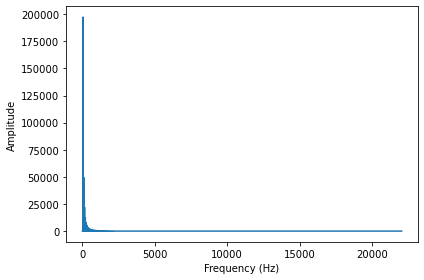
\includegraphics[width=0.75\textwidth]{sum4.png}
		\caption{С таким спектром}
		\label{fig:sum4}
	\end{figure}
	\begin{figure}[H]
		\centering
		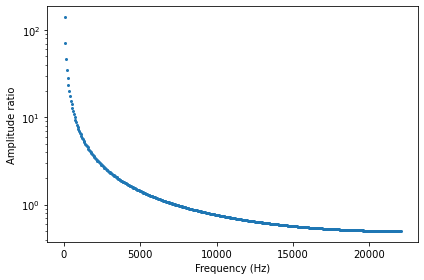
\includegraphics[width=0.75\textwidth]{sum5.png}
		\caption{Отношение значения выхода к значению входа}
		\label{fig:sum5}
	\end{figure}
	\begin{lstlisting}[language=Python,caption=Получение фильтра для суммирования]
		diff_window = np.array([1.0, -1.0])
		padded = zero_pad(diff_window, len(in_wave))
		diff_wave = Wave(padded, framerate = in_wave.framerate)
		diff_filter = diff_wave.make_spectrum()
		cumsum_filter = diff_filter.copy()
		cumsum_filter.hs[1:] = 1 / cumsum_filter.hs[1:]
		cumsum_filter.hs[0] = np.inf
	\end{lstlisting}
	\begin{lstlisting}[language=Python,caption=Сравнение суммирования и интегрирования]
		integ_filter = cumsum_filter.copy()
		integ_filter.hs[1:] = integ_filter.framerate / (PI2 * 1j * integ_filter.fs[1:])
		integ_filter.hs[0] = np.inf
		cumsum_filter.plot(label='cumsum filter', alpha=0.7)
		integ_filter.plot(label='integral filter', alpha=0.7)
		cumsum_filter.plot(label = 'cumsum filter')
		ratio_spectrum.plot(label='ratio', marker='.', ms=4, ls='')
	\end{lstlisting}
	\begin{figure}[H]
		\centering
		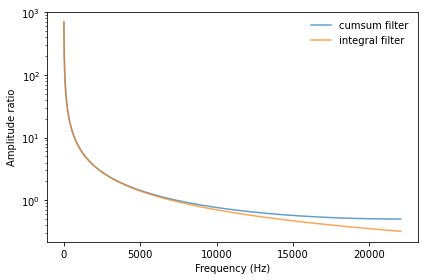
\includegraphics[width=0.75\textwidth]{sum6.png}
		\caption{Результат сравнения}
		\label{fig:sum6}
	\end{figure}
	\begin{figure}[H]
		\centering
		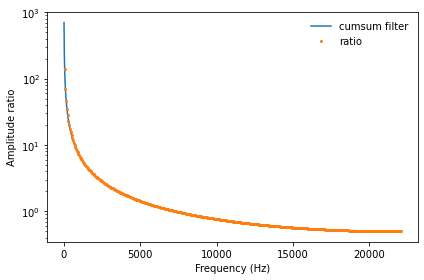
\includegraphics[width=0.75\textwidth]{sum7.png}
		\caption{Сравнение вычисленных соотношений с полученным фильтром}
		\label{fig:sum7}
	\end{figure}
	Они совпадают, подтверждая, что фильтр для суммирования является обратным разностному фильтру.	
	\begin{lstlisting}[language=Python,caption=Вычисляем выходной сигнал с помощью теоремы о свертке]
		out_wave.plot(label = 'summed', alpha = 0.7)
		cumsum_filter.hs[0] = 0
		out_wave2 = (in_spectrum * cumsum_filter).make_wave()
		out_wave2.plot(label = 'filtered', alpha = 0.7)
	\end{lstlisting}
	\begin{figure}[H]
		\centering
		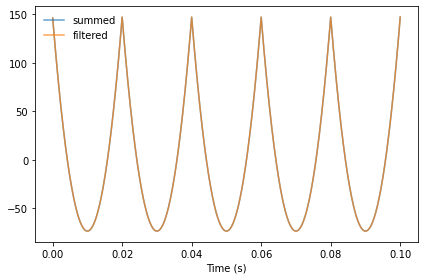
\includegraphics[width=0.75\textwidth]{sum8.png}
		\caption{Сравниваем результаты с спектром исходного сигнала}
		\label{fig:sum8}
	\end{figure}
	Разница между ними - примерно 0.
	
	\chapter{Упражнения}
	\section{Задание 1}
	Проверяем работу фильтра для суммирования с апериодическими сигналами.
	\begin{lstlisting}[language=Python,caption=Возьмем акции Facebook и повторим все действия из предыдущей главы]
		in_wave = close
		in_wave.unbias()
		in_wave.plot()
		in_spectrum = in_wave.make_spectrum()
		in_spectrum.plot()
		...
	\end{lstlisting}
	\begin{figure}[H]
		\centering
		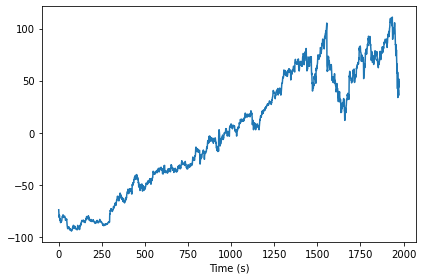
\includegraphics[width=0.75\textwidth]{test1.png}
		\caption{График цен}
		\label{fig:test1}
	\end{figure}
	\begin{figure}[H]
		\centering
		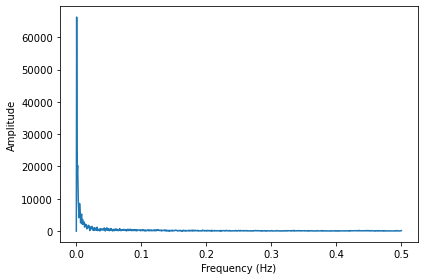
\includegraphics[width=0.75\textwidth]{test2.png}
		\caption{Спектр цен}
		\label{fig:test2}
	\end{figure}
	\begin{figure}[H]
		\centering
		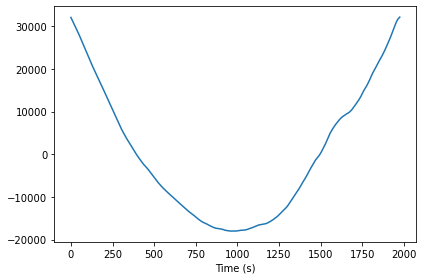
\includegraphics[width=0.75\textwidth]{test3.png}
		\caption{Посчитали нарастающую сумму}
		\label{fig:test3}
	\end{figure}
	\begin{figure}[H]
		\centering
		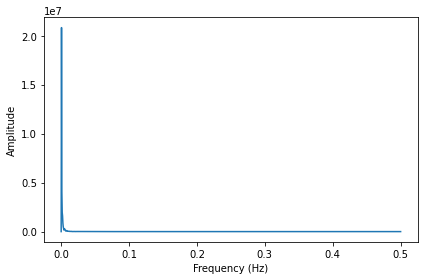
\includegraphics[width=0.75\textwidth]{test4.png}
		\caption{И получили вот такой спектр}
		\label{fig:test4}
	\end{figure}
	\begin{figure}[H]
		\centering
		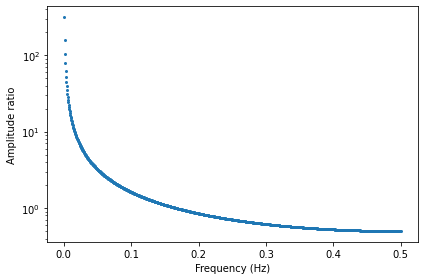
\includegraphics[width=0.75\textwidth]{test5.png}
		\caption{Отношение значения выхода к значению входа}
		\label{fig:test5}
	\end{figure}
	\begin{figure}[H]
		\centering
		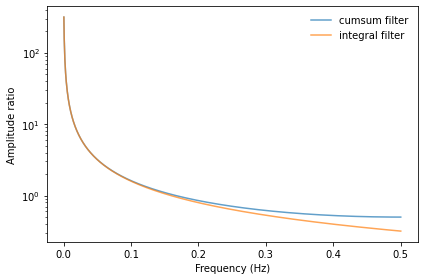
\includegraphics[width=0.75\textwidth]{test6.png}
		\caption{Результат сравнения двух фильтров}
		\label{fig:test6}
	\end{figure}
	\begin{figure}[H]
		\centering
		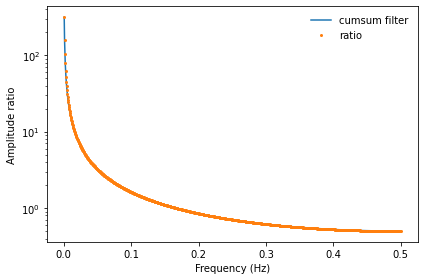
\includegraphics[width=0.75\textwidth]{test7.png}
		\caption{Сравнение вычисленных соотношений с результатом применения фильтра}
		\label{fig:test7}
	\end{figure}
	Они совпадают.
	\begin{figure}[H]
		\centering
		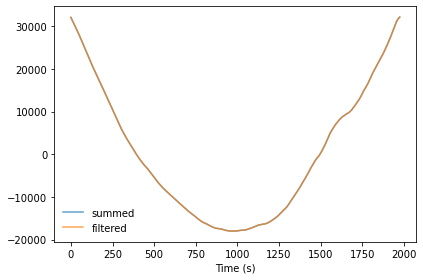
\includegraphics[width=0.75\textwidth]{test8.png}
		\caption{Сравниваем полученные результаты с спектром исходного сигнала}
		\label{fig:test8}
	\end{figure}
	Разница между ними близка к 0. Можно сделать вывод, что с апериодическими сигналами данный фильтр работает так же, как и с периодическими.

	\section{Задание 2}
	Сравнение \texttt{diff} и \texttt{differentiate} на примере треугольного сигнала.
	\begin{lstlisting}[language=Python,caption=И снова треугольный сигнал]
		from thinkdsp import TriangleSignal

		in_wave = TriangleSignal(freq = 50).make_wave(duration = 0.1, framerate = 44100)
		in_wave.plot()
		out_wave = in_wave.diff()
		out_wave.plot()
	\end{lstlisting}
	\begin{figure}[H]
		\centering
		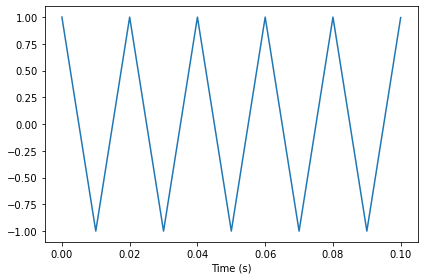
\includegraphics[width=0.75\textwidth]{task1.png}
		\caption{Треугольный сигнал (если вдруг кто забыл, как он выглядит)}
		\label{fig:task1}
	\end{figure}
	\begin{figure}[H]
		\centering
		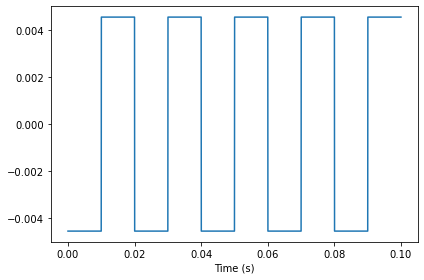
\includegraphics[width=0.75\textwidth]{task2.png}
		\caption{Применяем разностный фильтр}
		\label{fig:task2}
	\end{figure}
	Получился прямоугольный сигнал (немного неожиданно).
	\begin{lstlisting}[language=Python,caption=Применение фильтра для дифференцирования]
		out_result = in_wave.make_spectrum().differentiate()
		out_result.plot()
		out_wave2 = out_result.make_wave()
		out_wave2.plot()
	\end{lstlisting}
	\begin{figure}[H]
		\centering
		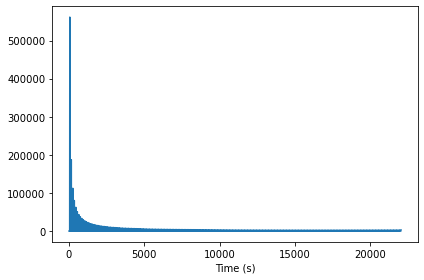
\includegraphics[width=0.75\textwidth]{task3.png}
		\caption{Полученный спектр сигнала}
		\label{fig:task3}
	\end{figure}
	\begin{figure}[H]
		\centering
		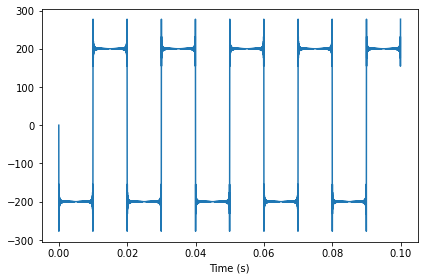
\includegraphics[width=0.75\textwidth]{task4.png}
		\caption{Сигнал после фильтра}
		\label{fig:task4}
	\end{figure}
	Тоже получили прямоугольный сигнал, но с более низким качеством. Проблема заключается в том, что производная не определена в вершинах треугольного сигнала.	

	\section{Задание 3}
	Сравнение \texttt{cumsum} и \texttt{integrate} на примере прямоугольного сигнала.
	\begin{lstlisting}[language=Python,caption=Прямоугольный сигнал]
		from thinkdsp import SquareSignal

		in_wave = SquareSignal(freq = 50).make_wave(duration=0.1, framerate=44100)
		in_wave.plot()
	\end{lstlisting}
	\begin{figure}[H]
		\centering
		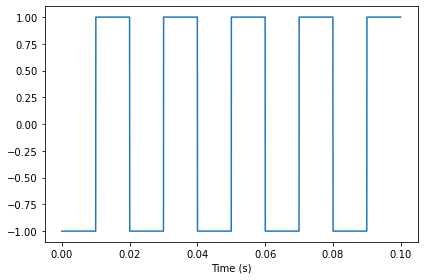
\includegraphics[width=0.75\textwidth]{task5.png}
		\caption{Прямоугольный сигнал}
		\label{fig:task5}
	\end{figure}
	\begin{lstlisting}[language=Python,caption=Сравнение двух фильтров]
		out_wave = in_wave.cumsum()
		spectrum = in_wave.make_spectrum().integrate()
		spectrum.hs[0] = 0
		out_wave2 = spectrum.make_wave()
		out_wave.unbias()
		out_wave.normalize()
		out_wave2.normalize()
		out_wave.plot()
		out_wave2.plot()
	\end{lstlisting}
	\begin{figure}[H]
		\centering
		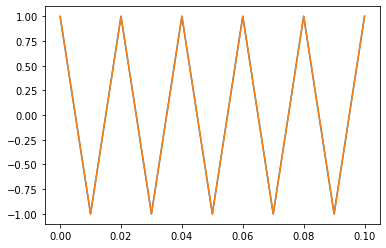
\includegraphics[width=0.75\textwidth]{task6.png}
		\caption{Сравнение результата работы двух фильтров}
		\label{fig:task6}
	\end{figure}
	Получился треугольный сигнал. Результаты этих двух фильтров совпадают небольшой точностью (всего 3 знака после запятой).

	\section{Задание 4}
	Применение двойного интегрирования на примере пилообразного сигнала.
	\begin{lstlisting}[language=Python,caption=Пилообразный сигнал]
		from thinkdsp import SawtoothSignal

		in_wave = SawtoothSignal(freq = 50).make_wave(duration=0.1, framerate=44100)
		in_wave.plot()
	\end{lstlisting}
	\begin{figure}[H]
		\centering
		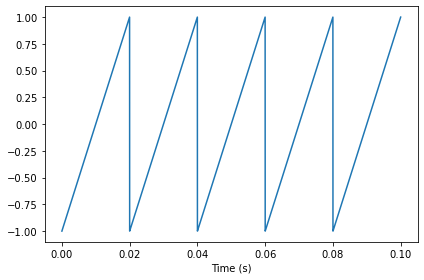
\includegraphics[width=0.75\textwidth]{task7.png}
		\caption{Это пилообразный сигнал}
		\label{fig:task7}
	\end{figure}
	\begin{lstlisting}[language=Python,caption=Два раза применили фильтр для суммирования]
		out_wave = in_wave.cumsum()
		out_wave.unbias()
		out_wave.plot()
		out_wave = out_wave.cumsum()
		out_wave.plot()
	\end{lstlisting}
	\begin{figure}[H]
		\centering
		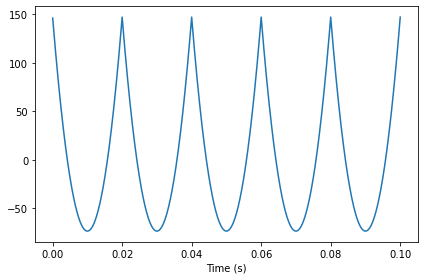
\includegraphics[width=0.75\textwidth]{task8.png}
		\caption{Первый раз - получилась парабола}
		\label{fig:task8}
	\end{figure}
	\begin{figure}[H]
		\centering
		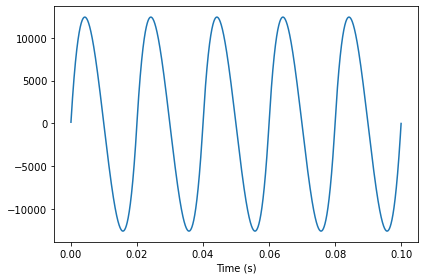
\includegraphics[width=0.75\textwidth]{task9.png}
		\caption{Второй раз - получилась кубическая кривая}
		\label{fig:task9}
	\end{figure}
	\begin{lstlisting}[language=Python,caption=Два раза интегрируем и строим спектр]
		spectrum = (in_wave.make_spectrum().integrate()).integrate()
		spectrum.hs[0] = 0
		out_wave2 = spectrum.make_wave()
		out_wave2.plot()
		out_wave2.make_spectrum().plot(high = 500)
	\end{lstlisting}
	\begin{figure}[H]
		\centering
		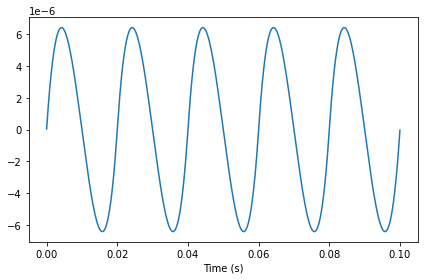
\includegraphics[width=0.75\textwidth]{task10.png}
		\caption{Также получили кубическую кривую}
		\label{fig:task10}
	\end{figure}
	Результат напоминает синусоиду, но это не она.
	\begin{figure}[H]
		\centering
		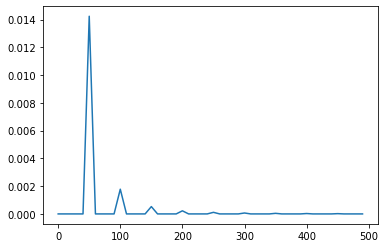
\includegraphics[width=0.75\textwidth]{task11.png}
		\caption{Спектр полученного сигнала}
		\label{fig:task11}
	\end{figure}
	Интегрирование действует как ФНЧ. После двух интегрирований мы отфильтровали почти все гармоники спектра, кроме фундаментальной.

	\section{Задание 5}
	Два раза применить разностный фильтр и фильтр для дифференцирования на примере кубического сигнала.
	\begin{lstlisting}[language=Python,caption=Кубический сигнал]
		from thinkdsp import CubicSignal

		in_wave = CubicSignal(freq = 0.0005).make_wave(duration=10000, framerate=1)
		in_wave.plot()
	\end{lstlisting}
	\begin{figure}[H]
		\centering
		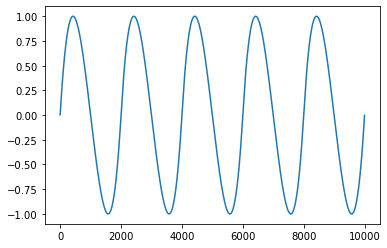
\includegraphics[width=0.75\textwidth]{task12.png}
		\caption{Кубический сигнал}
		\label{fig:task12}
	\end{figure}
	\begin{lstlisting}[language=Python,caption=Применение разностного фильтра]
		out_wave = in_wave.diff()
		out_wave.plot()
		out_wave = out_wave.diff()
		out_wave.plot()
	\end{lstlisting}
	\begin{figure}[H]
		\centering
		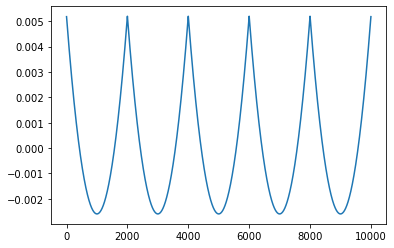
\includegraphics[width=0.75\textwidth]{task13.png}
		\caption{Первый раз - парабола}
		\label{fig:task13}
	\end{figure}
	\begin{figure}[H]
		\centering
		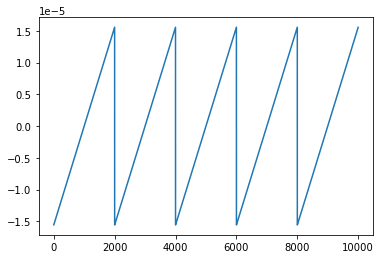
\includegraphics[width=0.75\textwidth]{task14.png}
		\caption{Второй раз - треугольный сигнал}
		\label{fig:task14}
	\end{figure}
	\begin{lstlisting}[language=Python,caption=Применение фильтра для дифференцирования]
		spectrum = in_wave.make_spectrum().differentiate().differentiate()
		out_wave2 = spectrum.make_wave()
		out_wave2.plot()
	\end{lstlisting}
	\begin{figure}[H]
		\centering
		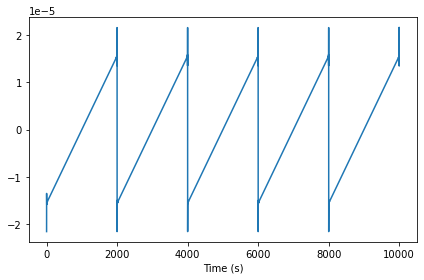
\includegraphics[width=0.75\textwidth]{task15.png}
		\caption{Результат двойного применения фильтра}
		\label{fig:task15}
	\end{figure}
	Получился пилообразный сигнал, но низкого качества. Производная параболического сигнала (после первого раза применения фильтра) в вершинах не определена.
	\begin{lstlisting}[language=Python,caption=Сравнение результатов работы фильтров]
		from thinkdsp import zero_pad, Wave

		diff_window = np.array([-1.0, 2.0, -1.0])
		padded = zero_pad(diff_window, len(in_wave))
		diff_wave = Wave(padded, framerate = in_wave.framerate)
		diff_filter = diff_wave.make_spectrum()
		deriv_filter = in_wave.make_spectrum()
		deriv_filter.hs = (np.pi*2*1j*deriv_filter.fs)**2
		diff_filter.plot(label = '2nd diff')
		deriv_filter.plot(label = '2nd deriv')
	\end{lstlisting}
	\begin{figure}[H]
		\centering
		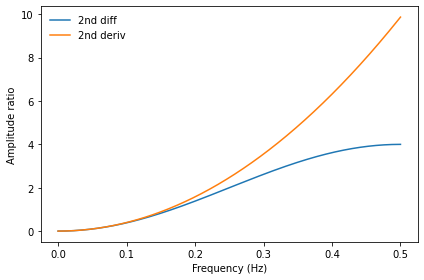
\includegraphics[width=0.75\textwidth]{task16.png}
		\caption{Результат сравнения}
		\label{fig:task16}
	\end{figure}
	Оба фильтра являются ФВЧ. 2-ая производная является параболической и хорошо усиливает высокие частоты. 2-разность является приближением 2-й производной только на низких частотах, а на высоких частотах она существенно отклоняется.

	\chapter{Вывод}
	В данной работе мы познакомились с методами дифференцирования (разности) и интегрирования (суммы) различных сигналов. Также посмотрели их работу с некоторыми сигналами.
\end{document}